% Created 2022-10-13 Thu 18:19
% Intended LaTeX compiler: pdflatex
\documentclass[11pt]{article}
\usepackage[utf8]{inputenc}
\usepackage[T1]{fontenc}
\usepackage{graphicx}
\usepackage{longtable}
\usepackage{wrapfig}
\usepackage{rotating}
\usepackage[normalem]{ulem}
\usepackage{amsmath}
\usepackage{amssymb}
\usepackage{capt-of}
\usepackage{hyperref}
\author{Alberto Valdez}
\date{\today}
\title{Statistical Tests\\\medskip
\large Notes on statistical tests with R}
\hypersetup{
 pdfauthor={Alberto Valdez},
 pdftitle={Statistical Tests},
 pdfkeywords={},
 pdfsubject={},
 pdfcreator={Emacs 28.1 (Org mode 9.6)}, 
 pdflang={English}}
\begin{document}

\maketitle
\tableofcontents


\section{Statistical Tests}
\label{sec:orgc7af203}

Due to the structured nature of statistical testing, if we can determine any two components of a statistical analysis (input variables, analytical question, or statistical test), we can infer the third. To simplify the process of inferring what component is needed, you can use a statistical test lookup table such as the following:

\begin{center}
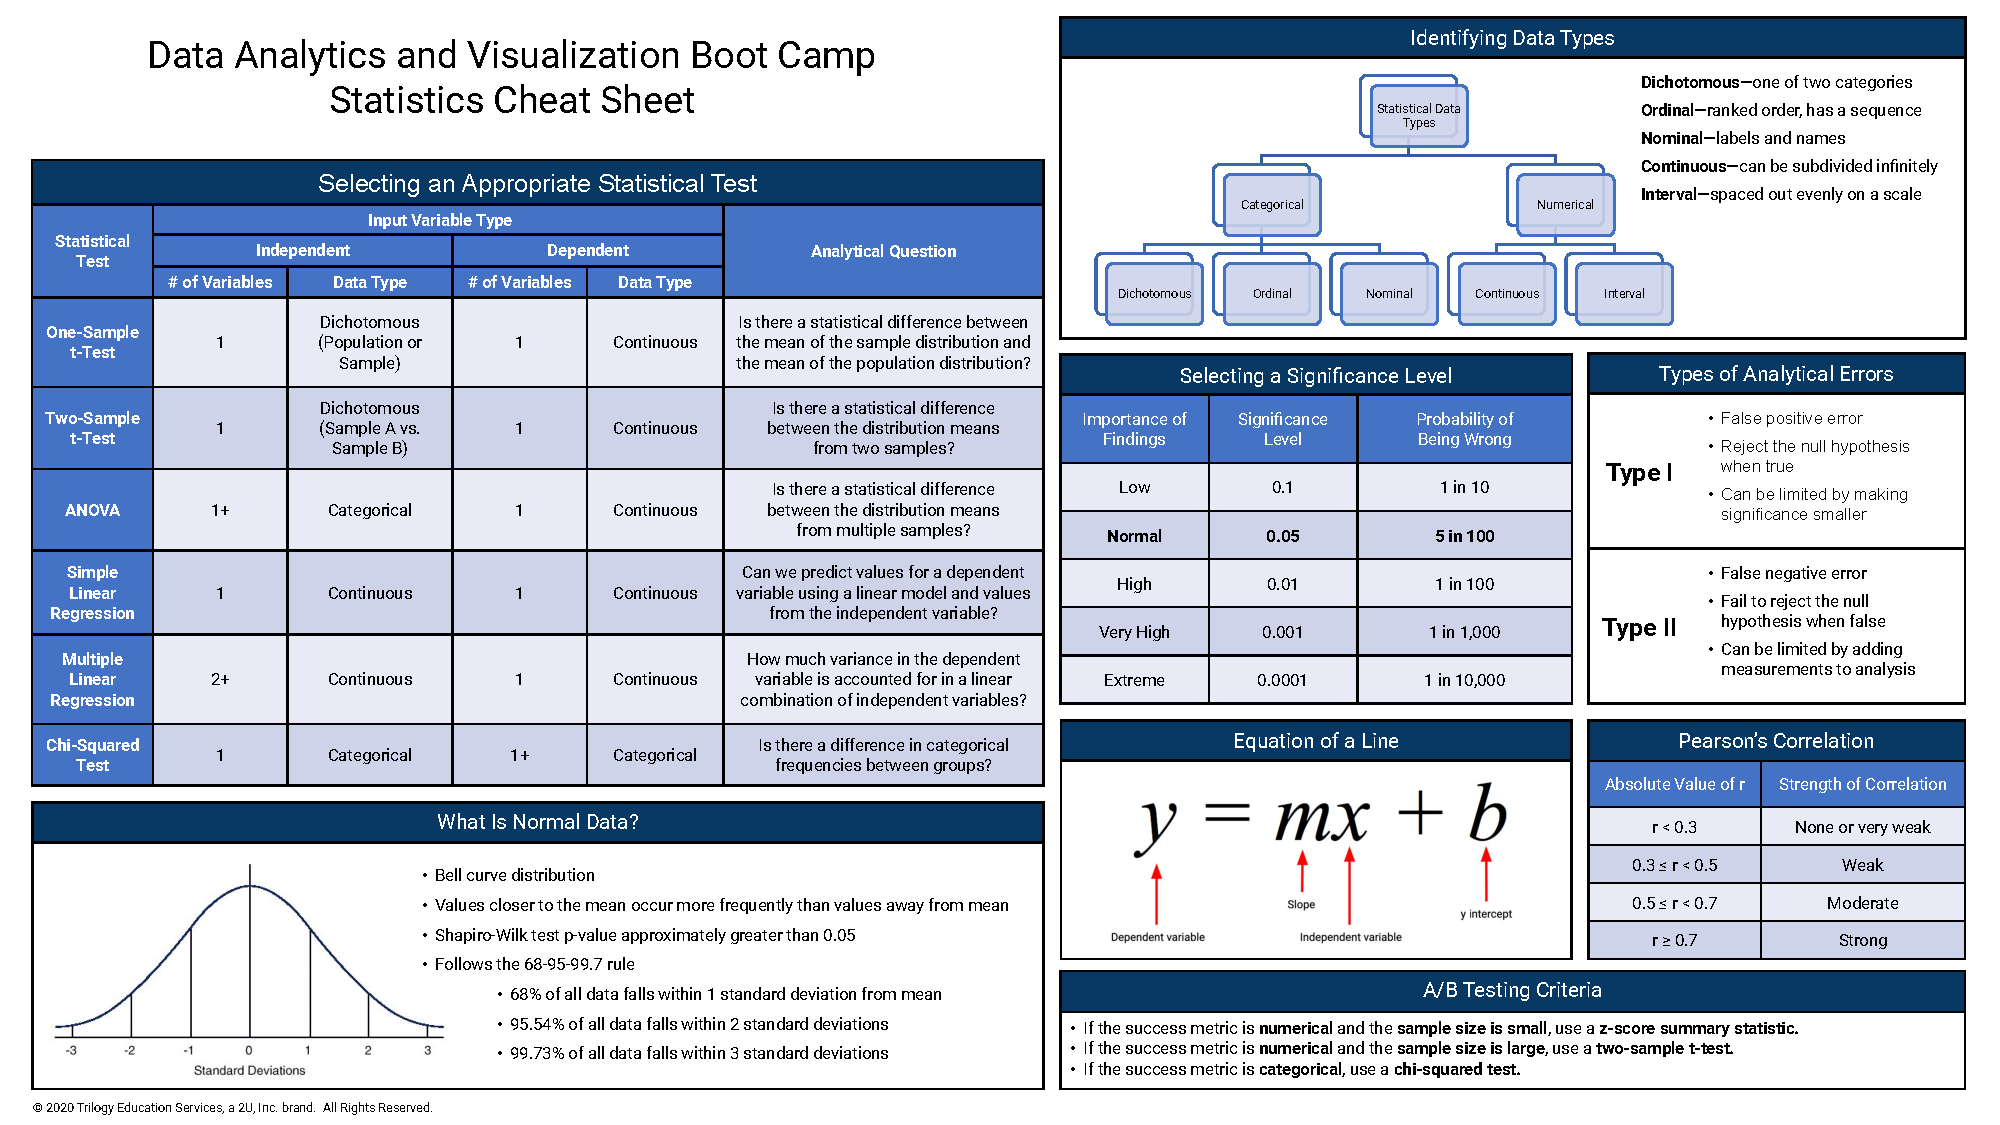
\includegraphics[width=.9\linewidth]{./resources/Stats_Cheat_Sheet.pdf}
\end{center}

There are two major data types in statistics: categorical and numerical. Within these types are several subtypes, each with its own use cases.

\begin{verbatim}
library(ggplot2)
library(tidyverse)
\end{verbatim}

\section{Data Type}
\label{sec:orgeed7e94}

\subsection{Categorical Data}
\label{sec:orgca4f2e1}

Represents data characteristics or qualitative descriptions, also known as qualitative data. Statistical tests that use it, employ it to inform which groups to compare.

\subsubsection{Dichotomous Data}
\label{sec:org5a9e146}

Data collected from either one of two categories. It can be in form of true/false Boolean values, two strings, etc.

\subsubsection{Ordinal Data}
\label{sec:org4069e80}

This data has a ranked order, but we don't necessarily know the value between each ordinal data point. It is popular because it allows for quantitative analysis without the need of machinery and tools to obtain measurements.

\subsubsection{Nominal Data}
\label{sec:orge910bbd}

Is data that is used as labels or names for other measures. Can be an identification number or can be a list of three options. It has no ranking and it is used in a more quantitative data type to perform an analysis.

\subsubsection{Numerical Data}
\label{sec:orge564293}

Obtained by taking a measurement from an instrument or by counting. It is used to perform quantitative analysis. Within numerical data there are two primary data types to consider: continuous and interval.

\subsubsection{Continuous Data}
\label{sec:org5e40c9f}

It can be subdivided infinitely. For example, measuring in centimeters, millimeters, nanometers, and so on. It is typically recorded with decimal places to match the precision of the measurement. Generates precise results.

\subsubsection{Interval Data}
\label{sec:org35c66d5}

Data spaced out evenly on a scale, also known as integer data, it doesn't use decimal places and can't be subdivided. It also can't be multiplied or divided. It can be easily grouped together or bucketed. Interval data can be treated as numerical data type and transformed into nominal data type.

\section{Distributions}
\label{sec:orgcd9e9ea}

Normal distribution, or normality, is commonly referred to as ``the bell curve'' as describes a dataset where values farther from its mean occur less frequenly than values closer to its mean.

In statistics, the central limit theorem is a key concept that states if you take sufficiently large samples of data from a dataset with mean μ (mu) and standard deviation σ (sigma), then the distribution will approximate normal distribution.

\subsection{Test for normality}
\label{sec:orgbdbea43}

\subsubsection{Qualitative Test}
\label{sec:orgb042113}

The qualitative test for normality is a visual assessment of the distribution of data, which looks for the characteristic bell curve shape across the distribution.

\begin{verbatim}
ggplot(mtcars,aes(x=wt)) +
  geom_density()
\end{verbatim}

\begin{org}
\begin{center}
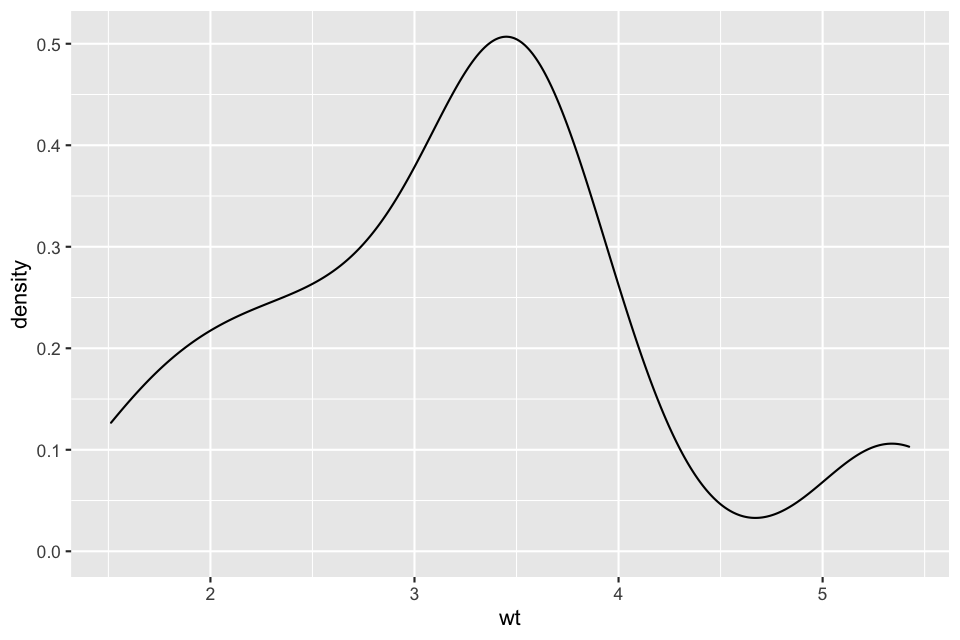
\includegraphics[width=.9\linewidth]{./resources/mtcars_density.png}
\end{center}
\end{org}

Geom density plots a numerical vector by creating buckets of similar values by calculating the density for each bucket.

The results of each bucket density calculation are plotted, connected, and smoothed out to create our distribution plot. Although our data distribution does not perfectly match the normal bell curve shape, the distribution does approximate a normal distribution and could be used for further analysis.

\subsubsection{Quantitative Test}
\label{sec:orgfc4a380}

The quantitative test for normality uses a statistical test to quantify the probability of whether or not the test data came from a normally distributed dataset.

The shapiro test function only requires the numeric vector of values you wish to test.

\begin{verbatim}
shapiro.test(mtcars$wt)
\end{verbatim}

\begin{org}


Shapiro-Wilk normality test

data:  mtcars\$wt
W = 0.94326, p-value = 0.09265
\end{org}

If our p-value is around 0.05 or more, we would say that our input data meets this assumption. But what happens if our data distribution does not look like a bell curve, or the p-value of the Shapiro-Wilk tests is too small?

\section{Skew}
\label{sec:org474f9f7}

When dealing with relatively smaller sample sizes, our data distributions are often asymmetrical. Compared to the normal distribution, where each tail of the distribution (on either side of the mean μ) mirrors one another, the asymmetrical distribution has one distribution tail that is longer than the other. This asymmetrical distribution is commonly referred to as a skewed distribution and there are two types—left skew and right skew.

\subsection{Managing Skewness}
\label{sec:orgf82ec5c}

If our dataset is large, or the skewness is very subtle, we would simply point out that our data distribution shows signs of skew during reporting or presentation. In these cases, our mean and median will be roughly the same value, and there should be minimal impact to any downstream analysis.

If our dataset is smaller, or the skewness does impact the overall shape of our distribution, more action is needed. There are a few different things we can try:

\begin{itemize}
\item If possible, add more data points to our dataset to alleviate the effect of skew. However, this might not be possible or might not improve the distribution.
\item Resample or regenerate data if we think that the data might not be representative of the original conditions or dataset.
\item Transform our data values by normalization, using another numerical variable, or by transforming the data using an operator.
\end{itemize}

\section{Hypothesis testing}
\label{sec:orgc048e02}

Regardless of the complexity of the dataset or the proposed question, hypothesis testing uses the same five steps:

\begin{enumerate}
\item Generate a null hypothesis, its corresponding alternate hypothesis, and the significance level.
\item Identify a statistical analysis to assess the truth of the null hypothesis.
\item Compute the p-value using statistical analysis.
\item Compare p-value to the significance level.
\item Reject (or fail to reject) the null hypothesis and generate the conclusion.

After determining which statistical analysis is most appropriate and analyzing our data, we must quantify our statistical results using probability. In our example, we are calculating probability directly; however, most statistical tests will produce probability in the form of a p-value.

The p-value, or probability value, tells us the likelihood that we would see similar results if we tested our data again, if the null hypothesis is true. Therefore, we use the p-value to provide quantitative evidence as to which of our hypotheses are true.
\end{enumerate}

\subsection{Tails}
\label{sec:org7b99bc3}

When it comes to checking our statistical tests, the documentation will tell us if our statistical test is one-tailed or two-tailed. Once we have determined the number of tails considered for both our hypotheses and statistical test, we can determine if we need to adjust our p-value:

\begin{itemize}
\item If our hypotheses and statistical test are both two-tailed, use the statistical test p-value as is.
\item If our hypotheses are one-tailed, but our statistical test is two-tailed, divide the statistical test p-value by 2.
\end{itemize}

\subsection{Error in Hypothesis Testing}
\label{sec:orgcc8e273}

In an ideal world, we would be able to definitively decide if our null hypothesis or alternative hypothesis was true by collecting all possible measurements or data points. But since this is often impossible, we must approximate truth using a subset of data.

In most cases, our approximations and hypothesis selection will be correct and represent the true real-world results. But due to the variability of data, at some point our hypothesis selection will be incorrect. Our incorrect hypothesis selection can fall into two categories:

\begin{itemize}
\item Type I error (also known as a false positive error)—an error in which we reject the null hypothesis when it is actually true. In other words, the observations and measurements used in our statistical test should have been attributed to random chance, but we attributed them to something else.
\item Type II error (also known as a false negative error)—an error in which we fail to reject the null hypothesis when it is actually false. In other words, our analysis demonstrates that the observations were due to random chance, but they were not. The observations and measurements used in our statistical test failed to reflect an external force or influence to our problem.
\end{itemize}

When it comes to limiting our type I and type II errors, there are two basic methods:

\begin{itemize}
\item A type I error can be limited by making your significance level smaller. A smaller significance level makes it harder to accidentally reject the null hypothesis when the data was truly random. This is also why our significance level (alpha or ɑ) is sometimes referred to as our false positive rate.
\item A type II error can be limited by increasing the power of the analysis. Although performing a power analysis is outside the scope of the course, power can be increased by adding additional measurements or observations to our analysis.
\end{itemize}

\subsection{Steps}
\label{sec:org49e288e}

\begin{enumerate}
\item Generate a null Hypothesis, its corresponding alternate hypothesis, and the significance level.
\item Identify a statistical analysis to assess the truth of the null hypothesis.
\item Compute the p-value using statistical analysis.
\item Compare p-value to the significance level.
\item Reject (or fail to reject) the null hypothesis and generate the conclusion.
\end{enumerate}

\section{Analysis of Mean in R}
\label{sec:orgeb5194e}

We will use the sample and sample n functions.

Using the sample\textsubscript{n}()function only requires two arguments:

\begin{itemize}
\item tbl is the name of the input table, which is typically the name of a data frame. Optionally, we can use a dplyr pipe (\%>\%) to provide the data frame object directly, in which case, this argument is optional.
\item size is the number of rows to return. As noted in the documentation, if we are providing a data frame that was grouped using the group\textsubscript{by}()function, the size argument is the number of groups to return.
\end{itemize}

\begin{verbatim}
population_table <-
  read.csv(
    'used_car_data.csv',
    check.names = F,
    stringsAsFactors = F
)
population_table %>% head
\end{verbatim}

\begin{org}
\begin{center}
\begin{tabular}{lrrrrlllr}
Car\textsubscript{Name} & Year & Selling\textsubscript{Price} & Present\textsubscript{Price} & Miles\textsubscript{Driven} & Fuel\textsubscript{Type} & Seller\textsubscript{Type} & Transmission & Owner\\
\hline
ritz & 2014 & 3350 & 5590 & 27000 & Petrol & Dealer & Manual & 0\\
sx4 & 2013 & 4750 & 9540 & 43000 & Diesel & Dealer & Manual & 0\\
ciaz & 2017 & 7250 & 9850 & 6900 & Petrol & Dealer & Manual & 0\\
wagon r & 2011 & 2850 & 4150 & 5200 & Petrol & Dealer & Manual & 0\\
swift & 2014 & 4600 & 6870 & 42450 & Diesel & Dealer & Manual & 0\\
vitara brezza & 2018 & 9250 & 9830 & 2071 & Diesel & Dealer & Manual & 0\\
\end{tabular}
\end{center}
\end{org}

Then we can plot it with density.

\begin{verbatim}
plt <-
  ggplot(population_table, aes(x=log10(Miles_Driven)))
plt +
  geom_density()
\end{verbatim}

\begin{org}
\begin{center}
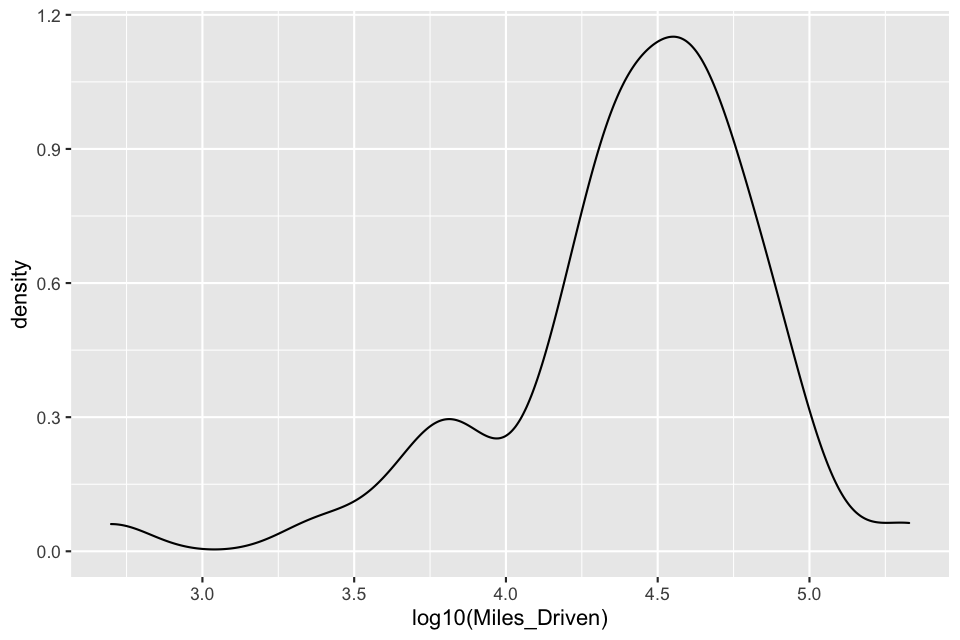
\includegraphics[width=.9\linewidth]{./resources/used_car_density.png}
\end{center}
\end{org}

Now that we characterized our population data using our density plot, we'll create a sample dataset using dplyr's sample n function.

We will randomly sample 50 datapoints.
\begin{verbatim}
sample_table <- population_table %>% sample_n(50)
plt <-
  ggplot(sample_table, aes(x=log10(Miles_Driven)))
plt + geom_density()
\end{verbatim}

\begin{org}
\begin{center}
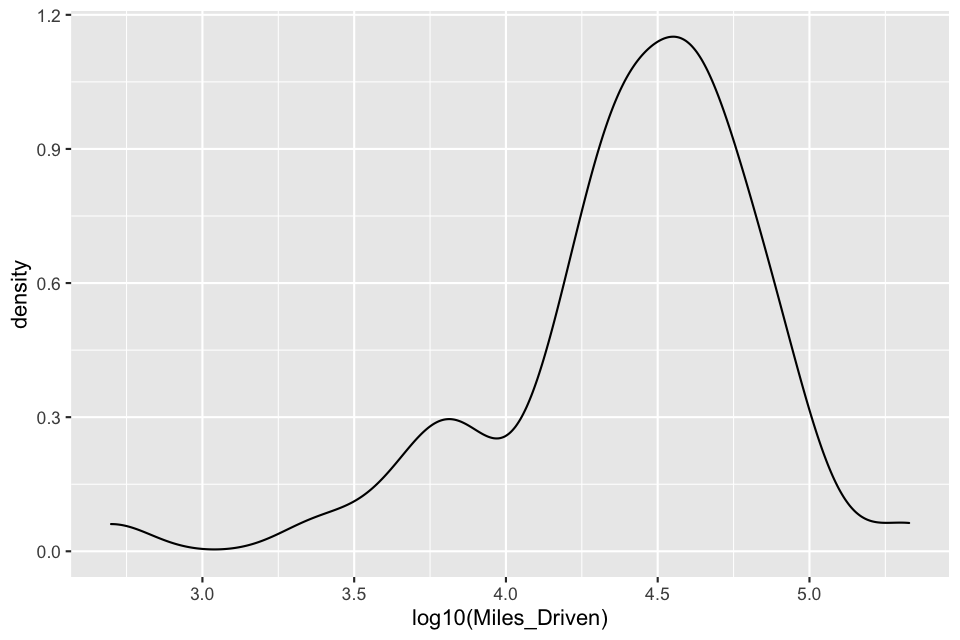
\includegraphics[width=.9\linewidth]{./resources/used_car_density.png}
\end{center}
\end{org}

Depending on the size of the population data, we may need to also adjust the size argument in our sample\textsubscript{n}() function to ensure that our sample data is representative of the underlying population data. There are two basic ways to check that our sample data is representative of the underlying population: a qualitative assessment of each density plot or a quantitative statistical test such as the one-sample t-test.

\subsection{One-Sample t-test}
\label{sec:org01515e9}

We are going to use the t test function to compare both sample and population means.

\begin{verbatim}
t.test(
  log10(sample_table$Miles_Driven),
  mu=mean(log10(population_table$Miles_Driven))
  )
\end{verbatim}

\begin{org}


One Sample t-test

data:  log10(sample\textsubscript{table}\$Miles\textsubscript{Driven})
t = 0.18735, df = 49, p-value = 0.8522
alternative hypothesis: true mean is not equal to 4.39449
95 percent confidence interval:
 4.278097 4.534815
sample estimates:
mean of x
 4.406456
\end{org}

The metric we are interested in is \textbf{p-value}. Assumming a significance level of 5 percent, our \textbf{p-value} is above it, therefore we don't have sufficient evidence to reject the null hypothesis and we would state that the two means are similar statistically.

\subsection{Two-Sample t-Test}
\label{sec:orgc1d19c1}

The second main form of the t-Test is a two-sample t-Test. Instead of testing whether a sample mean is statistically different from its population mean, the two-sample t-Test determines whether the means of two samples are statistically different.

\begin{verbatim}
sample_table <-
  population_table %>% sample_n(50)
head(sample_table)
\end{verbatim}

\begin{org}
\begin{center}
\begin{tabular}{lrrrrlllr}
Car\textsubscript{Name} & Year & Selling\textsubscript{Price} & Present\textsubscript{Price} & Miles\textsubscript{Driven} & Fuel\textsubscript{Type} & Seller\textsubscript{Type} & Transmission & Owner\\
\hline
ciaz & 2015 & 6750 & 8120 & 18796 & Petrol & Dealer & Manual & 0\\
fortuner & 2014 & 18750 & 35960 & 78000 & Diesel & Dealer & Automatic & 0\\
corolla altis & 2009 & 3600 & 15040 & 70000 & Petrol & Dealer & Automatic & 0\\
fortuner & 2015 & 23000 & 30610 & 40000 & Diesel & Dealer & Automatic & 0\\
verna & 2013 & 5110 & 9400 & 36198 & Petrol & Dealer & Automatic & 0\\
Yamaha FZ S V 2.0 & 2015 & 480 & 840 & 23000 & Petrol & Individual & Manual & 0\\
\end{tabular}
\end{center}
\end{org}

\begin{verbatim}
sample_table2 <-
  population_table %>% sample_n(50)
head(sample_table2)
\end{verbatim}

\begin{org}
\begin{center}
\begin{tabular}{lrrrrlllr}
Car\textsubscript{Name} & Year & Selling\textsubscript{Price} & Present\textsubscript{Price} & Miles\textsubscript{Driven} & Fuel\textsubscript{Type} & Seller\textsubscript{Type} & Transmission & Owner\\
\hline
creta & 2016 & 12900 & 13600 & 35934 & Diesel & Dealer & Manual & 0\\
Yamaha FZ  v 2.0 & 2015 & 600 & 840 & 29000 & Petrol & Individual & Manual & 0\\
city & 2016 & 10900 & 13600 & 30753 & Petrol & Dealer & Automatic & 0\\
fortuner & 2017 & 33000 & 36230 & 6000 & Diesel & Dealer & Automatic & 0\\
grand i10 & 2015 & 4850 & 5700 & 21125 & Diesel & Dealer & Manual & 0\\
fortuner & 2015 & 23000 & 30610 & 40000 & Diesel & Dealer & Automatic & 0\\
\end{tabular}
\end{center}
\end{org}

Now we compare both samples.
\begin{verbatim}
t.test(
  log10(sample_table$Miles_Driven),
  log10(sample_table2$Miles_Driven)
)
\end{verbatim}

\begin{org}


Welch Two Sample t-test

data:  log10(sample\textsubscript{table}\$Miles\textsubscript{Driven}) and log10(sample\textsubscript{table2}\$Miles\textsubscript{Driven})
t = 0.092572, df = 97.815, p-value = 0.9264
alternative hypothesis: true difference in means is not equal to 0
95 percent confidence interval:
 -0.1510382  0.1658187
sample estimates:
mean of x mean of y
 4.359795  4.352405
\end{org}

We have failed to negate the null hypothesis once again as the p-value is not under 0.05.

However, two-sample t-tests are flexible and can be used for another purpose: to compare two samples, each from a different population.

\texttt{paired} tells the t.test() function to perform a paired t-test. This value must be set to TRUE.

\subsection{Comparing Samples}
\label{sec:orga844666}

Loading our new data.

\begin{verbatim}
mpg_data <- read.csv('mpg_modified.csv')
head(mpg_data)
\end{verbatim}

\begin{org}
\begin{center}
\begin{tabular}{llrrrlrrrll}
manufacturer & model & displ & year & cyl & trans & drv & cty & hwy & fl & class\\
\hline
audi & a4 & 1.8 & 1999 & 4 & auto(l5) & f & 18 & 29 & p & compact\\
audi & a4 & 2 & 2008 & 4 & manual(m6) & f & 20 & 31 & p & compact\\
audi & a4 quattro & 1.8 & 1999 & 4 & manual(m5) & 4 & 18 & 26 & p & compact\\
audi & a4 quattro & 2 & 2008 & 4 & manual(m6) & 4 & 20 & 28 & p & compact\\
audi & a6 quattro & 2.8 & 1999 & 6 & auto(l5) & 4 & 15 & 24 & p & midsize\\
audi & a6 quattro & 3.1 & 2008 & 6 & auto(s6) & 4 & 17 & 25 & p & midsize\\
\end{tabular}
\end{center}
\end{org}

Generate two data samples.

\begin{verbatim}
mpg_1999 <- mpg_data %>% filter(year==1999)
mpg_2008 <-mpg_data %>% filter(year==2008)
\end{verbatim}

\begin{org}
\end{org}

Measure whether there is a statistical difference in overall highway fuel efficiency between vehicles manufactured in 1999 versus 2008.

\begin{verbatim}
t.test(mpg_1999$hwy, mpg_2008$hwy, paired = T)
\end{verbatim}

\begin{org}


Paired t-test

data:  mpg\textsubscript{1999}\$hwy and mpg\textsubscript{2008}\$hwy
t = -1.1165, df = 37, p-value = 0.2714
alternative hypothesis: true mean difference is not equal to 0
95 percent confidence interval:
 -2.1480860  0.6217702
sample estimates:
mean difference
     -0.7631579
\end{org}

Here we fail to reject the null hypothesis once again.

\subsection{ANOVA Testing}
\label{sec:org15b4bee}

When dealing with large real-world numerical data, we're often interested in comparing the means across more than two samples or groups. The most straightforward way to do this is to use the analysis of variance (ANOVA) test, which is used to compare the means of a continuous numerical variable across a number of groups (or factors in R).

Depending on your dataset and questions you wish to answer, an ANOVA can be used in multiple ways. For the purposes of this course, we'll concentrate on two different types of ANOVA tests:

\begin{itemize}
\item A one-way ANOVA is used to test the means of a single dependent variable across a single independent variable with multiple groups. (e.g., fuel efficiency of different cars based on vehicle class).
\item A two-way ANOVA does the same thing, but for two different independent variables (e.g., vehicle braking distance based on weather conditions and transmission type).
\end{itemize}

Additionally, both ANOVA tests have assumptions about the input data that must be validated prior to using the statistical test:

\begin{enumerate}
\item The dependent variable is numerical and continuous, and the independent variables are categorical.
\item The dependent variable is considered to be normally distributed.
\item The variance among each group should be very similar.
\end{enumerate}

Unlike the t.test() function, where each group was a separate numeric vector, the aov() function expects that all of the observations and grouping information are contained within a single data frame.

For this statistical test, we'll answer the question, ``Is there any statistical difference in the horsepower of a vehicle based on its engine type?''

In this case, we will use the ``hp'' and ``cyl'' columns from our mtcars dataset. However, in the mtcars dataset, the cyl is considered a numerical interval vector, not a categorical vector. Therefore, we must clean our data before we begin, using the following code:

We will convert numeric column to factor.

\begin{verbatim}
mtcars_filt <- mtcars[,c("hp","cyl")]
mtcars_filt$cyl <- factor(mtcars_filt$cyl)
head(mtcars['cyl'])
\end{verbatim}

\begin{org}
\begin{center}
\begin{tabular}{r}
cyl\\
\hline
6\\
6\\
4\\
6\\
8\\
6\\
\end{tabular}
\end{center}
\end{org}

Now we can use ANOVA to compare means across multiple levels.

\begin{verbatim}
aov(hp ~ cyl, data=mtcars_filt)
\end{verbatim}

\begin{org}
Call:
   aov(formula = hp \textasciitilde{} cyl, data = mtcars\textsubscript{filt})

Terms:
                      cyl Residuals
Sum of Squares  104030.54  41696.33
Deg. of Freedom         2        29

Residual standard error: 37.91839
Estimated effects may be unbalanced
\end{org}

To retrieve our p-values, we have to wrap our aov()function in a summary() function as follows.

\begin{verbatim}
summary(aov(hp ~ cyl, data=mtcars_filt))
\end{verbatim}

\begin{org}
            Df Sum Sq Mean Sq F value   Pr(>F)
cyl          2 104031   52015   36.18 1.32e-08 \textbf{*}
Residuals   29  41696    1438
---
Signif. codes:  0 ‘***’ 0.001 ‘**’ 0.01 ‘*’ 0.05 ‘.’ 0.1 ‘ ’ 1
\end{org}

For our purposes, we are only concerned with the ``Pr(>F)'' column, which is the same as our p-value statistic.

In this case, our p-value is 1.32 ✕ 10\textsuperscript{-8}\^{}, which is much smaller than our assumed 0.05 percent significance level. Therefore, we would state that there is sufficient evidence to reject the null hypothesis and accept that there is a significant difference in horsepower between at least one engine type and the others.

\section{Correlation}
\label{sec:org77b8abf}

Correlation in statistics is the relationship between variable A and variable B. It is quantified by calculating a correlation coefficient, and the most common correlation coefficient is the Pearson correlation coefficient. The Pearson correlation coefficient is denoted as ``r'' in mathematics and is used to quantify a linear relationship between two numeric variables. The Pearson correlation coefficient ranges between -1 and 1, depending on the direction of the linear relationship.

\begin{center}
\begin{tabular}{ll}
Absolute Value of r & Strength of Correlation\\
\hline
r < 0.3 & None or very weak\\
0.3 ≤ r < 0.5 & Weak\\
0.5 ≤ r < 0.7 & Moderate\\
r ≥ 0.7 & Strong\\
\end{tabular}
\end{center}

We can use the \texttt{cor()} function to perform correlation analysis between two numeric variables.

We are going to use the \texttt{mtcars} dataset.

\begin{verbatim}
head(mtcars)
\end{verbatim}

\begin{org}
\begin{center}
\begin{tabular}{rrrrrrrrrrr}
mpg & cyl & disp & hp & drat & wt & qsec & vs & am & gear & carb\\
\hline
21 & 6 & 160 & 110 & 3.9 & 2.62 & 16.46 & 0 & 1 & 4 & 4\\
21 & 6 & 160 & 110 & 3.9 & 2.875 & 17.02 & 0 & 1 & 4 & 4\\
22.8 & 4 & 108 & 93 & 3.85 & 2.32 & 18.61 & 1 & 1 & 4 & 1\\
21.4 & 6 & 258 & 110 & 3.08 & 3.215 & 19.44 & 1 & 0 & 3 & 1\\
18.7 & 8 & 360 & 175 & 3.15 & 3.44 & 17.02 & 0 & 0 & 3 & 2\\
18.1 & 6 & 225 & 105 & 2.76 & 3.46 & 20.22 & 1 & 0 & 3 & 1\\
\end{tabular}
\end{center}
\end{org}

We will create a scatter plot.

\begin{verbatim}
plt <- ggplot(mtcars, aes(x=hp, y=qsec))
plt + geom_point()
\end{verbatim}

\begin{org}
\begin{center}
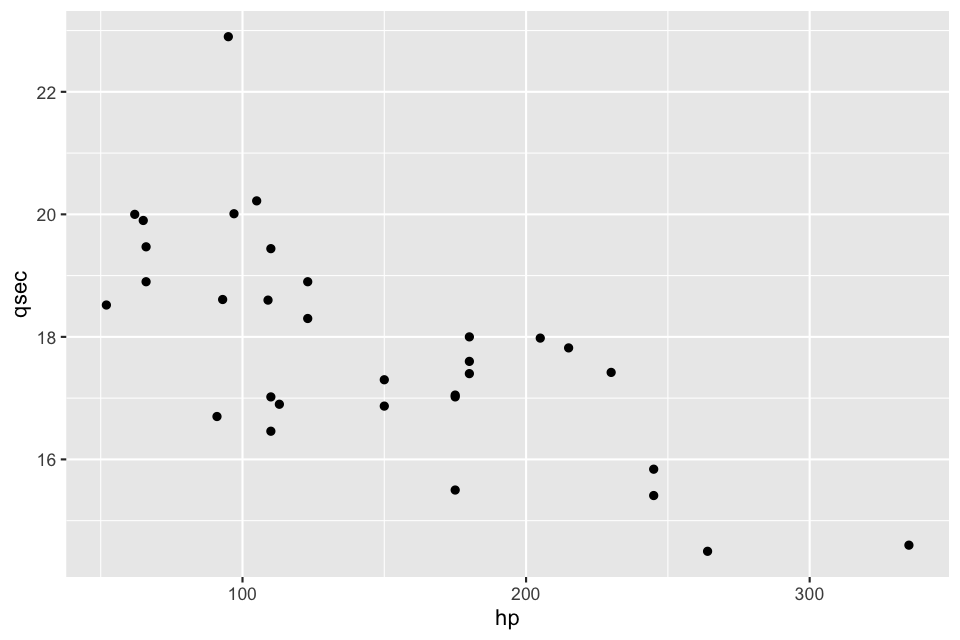
\includegraphics[width=.9\linewidth]{./resources/mtcars_cor1.png}
\end{center}
\end{org}

Looks like the quarter-mile time is negatively correlated with horsepower.

Let's verify it.

\begin{verbatim}
cor(mtcars$hp, mtcars$qsec)
\end{verbatim}

\begin{org}
\begin{center}
\begin{tabular}{r}
x\\
\hline
-0.708223388861953\\
\end{tabular}
\end{center}
\end{org}

\subsection{Car data correlation}
\label{sec:orgff120e9}

\begin{verbatim}
used_cars <-
  read.csv('used_car_data.csv', stringsAsFactors=F)
head(used_cars)
\end{verbatim}

\begin{org}
\begin{center}
\begin{tabular}{lrrrrlllr}
Car\textsubscript{Name} & Year & Selling\textsubscript{Price} & Present\textsubscript{Price} & Miles\textsubscript{Driven} & Fuel\textsubscript{Type} & Seller\textsubscript{Type} & Transmission & Owner\\
\hline
ritz & 2014 & 3350 & 5590 & 27000 & Petrol & Dealer & Manual & 0\\
sx4 & 2013 & 4750 & 9540 & 43000 & Diesel & Dealer & Manual & 0\\
ciaz & 2017 & 7250 & 9850 & 6900 & Petrol & Dealer & Manual & 0\\
wagon r & 2011 & 2850 & 4150 & 5200 & Petrol & Dealer & Manual & 0\\
swift & 2014 & 4600 & 6870 & 42450 & Diesel & Dealer & Manual & 0\\
vitara brezza & 2018 & 9250 & 9830 & 2071 & Diesel & Dealer & Manual & 0\\
\end{tabular}
\end{center}
\end{org}

Then we will plot the data to look for a correlation.

\begin{verbatim}
plt <-
  ggplot(
    used_cars,
    aes(x=Miles_Driven, y=Selling_Price)
)
plt + geom_point()
\end{verbatim}

\begin{org}
\begin{center}
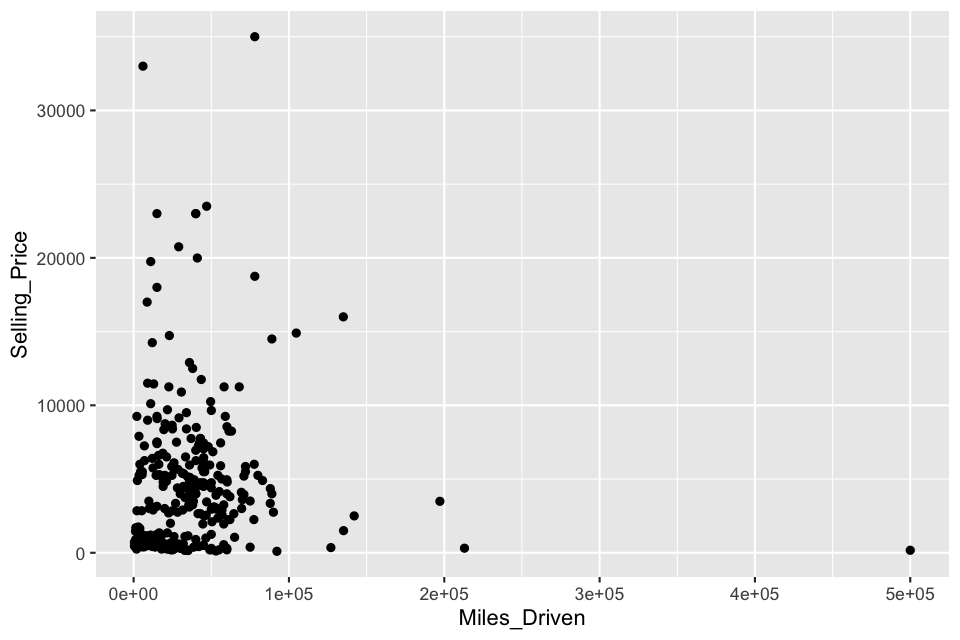
\includegraphics[width=.9\linewidth]{./resources/cars_corr.png}
\end{center}
\end{org}

This is not a clear answer. Let's try using cor.

\begin{verbatim}
cor(used_cars$Miles_Driven, used_cars$Selling_Price)
\end{verbatim}

\begin{org}
\begin{center}
\begin{tabular}{r}
x\\
\hline
0.0291870906742913\\
\end{tabular}
\end{center}
\end{org}

The correlation is negigible between miles driven and selling price.

Instead of computing each pairwise correlation, we can use the cor() function to produce a correlation matrix. A correlation matrix is a lookup table where the variable names of a data frame are stored as rows and columns, and the intersection of each variable is the corresponding Pearson correlation coefficient.

\begin{verbatim}
used_matrix <-
  as.matrix(
    used_cars[,c(
      "Selling_Price",
      "Present_Price",
      "Miles_Driven"
    )]
)
cor(used_matrix)
\end{verbatim}

\begin{org}
\begin{center}
\begin{tabular}{rrr}
Selling\textsubscript{Price} & Present\textsubscript{Price} & Miles\textsubscript{Driven}\\
\hline
1 & 0.878982545161495 & 0.0291870906742913\\
0.878982545161495 & 1 & 0.203647034009132\\
0.0291870906742913 & 0.203647034009132 & 1\\
\end{tabular}
\end{center}
\end{org}

If we look at the correlation matrix using either rows or columns, we can identify pairs of variables with strong correlation (such as selling price versus present price), or no correlation (like our previous example of miles driven versus selling price).
The correlation matrix is a very powerful data exploration tool that allows an analyst to scan large numerical datasets for variables of interest. Once the variables of interest have been identified, the analyst can move on to more rigorous data analysis and hypothesis testing.

\section{Linear Regression}
\label{sec:orgaeeecf9}

Linear regression is a statistical model that is used to predict a continuous dependent variable based on one or more independent variables fitted to the equation of a line.

y = mx + b

\begin{itemize}
\item Simple linear regression builds a linear regression model with one independent variable.
\item Multiple linear regression builds a linear regression model with two or more independent variables.
\end{itemize}

Linear regression tests the following hypotheses:

\begin{itemize}
\item H0 : The slope of the linear model is zero, or m = 0
\item Ha : The slope of the linear model is not zero, or m ≠ 0
\end{itemize}

If there is no significant linear relationship, each dependent value would be determined by random chance and error. Therefore, our linear model would be a flat line with a slope of 0.

To quantify how well our linear model can be used to predict future observations, our linear regression functions will calculate an r-squared value. The r-squared (r2) value is also known as the coefficient of determination and represents how well the regression model approximates real-world data points.

By combining the p-value of our hypothesis test with the r-squared value, the linear regression model becomes a powerful statistics tool that both quantifies a relationship between variables and provides a meaningful model to be used in any decision-making process.

Similar to our t-test analysis, there are a few assumptions about our input data that must be met before we perform our statistical analysis:

\begin{enumerate}
\item The input data is numerical and continuous.
\item The input data should follow a linear pattern.
\item There is variability in the independent x variable. This means that there must be more than one observation in the x-axis and they must be different values.
\item The residual error (the distance from each data point to the line) should be normally distributed.
\end{enumerate}

\subsection{Linear Regression in R}
\label{sec:org3ee0ac1}

Our previous correlation coefficient \texttt{r-value} in the mtcars dataset was high. So we can expect the linear model to perform well.

\begin{verbatim}
lm(qsec ~ hp, mtcars)
\end{verbatim}

\begin{org}


Call:
lm(formula = qsec \textasciitilde{} hp, data = mtcars)

Coefficients:
(Intercept)           hp
   20.55635     -0.01846
\end{org}

The \texttt{lm()} function returns our y intercent and the slope (hp) coefficient. Therefore, the linear regression model for our dataset would be the following.

qsec = -0.02hp + 20.56

Not let's summarize it to get the \texttt{p-value} and the \texttt{r-squared}.

\begin{verbatim}
summary(lm(qsec~hp, mtcars))
\end{verbatim}

\begin{org}


Call:
lm(formula = qsec \textasciitilde{} hp, data = mtcars)

Residuals:
    Min      1Q  Median      3Q     Max
-2.1766 -0.6975  0.0348  0.6520  4.0972

Coefficients:
             Estimate Std. Error t value Pr(>|t|)
(Intercept) 20.556354   0.542424  37.897  < 2e-16 \textbf{*}
hp          -0.018458   0.003359  -5.495 5.77e-06 \textbf{*}
---
Signif. codes:  0 ‘***’ 0.001 ‘**’ 0.01 ‘*’ 0.05 ‘.’ 0.1 ‘ ’ 1

Residual standard error: 1.282 on 30 degrees of freedom
Multiple R-squared:  0.5016,	Adjusted R-squared:  0.485
F-statistic: 30.19 on 1 and 30 DF,  p-value: 5.766e-06
\end{org}

The values are under \textbf{Multiple R-squared} and \textbf{p-value}.

\subsection{Results}
\label{sec:org982297a}

From our linear regression model, the r-squared value is 0.50, which means that roughly 50\% of the variablilty of our dependent variable (quarter-mile time predictions) is explained using this linear model. Compared to the Pearson correlation coefficient between quarter-mile race time and horsepower of -0.71, we can confirm that our r-squared value is approximately the square of our r-value. In a simple linear regression model, the higher the correlation is between two variables, the more that one variable can explain/predict the value of the other.

In addition, the p-value of our linear regression analysis is 5.77 x 10-6, which is much smaller than our assumed significance level of 0.05\%. Therefore, we can state that there is sufficient evidence to reject our null hypothesis, which means that the slope of our linear model is not zero.

Once we have calculated our linear regression model, we can visualize the fitted line against our dataset using ggplot2.

Calculate the data points.

\begin{verbatim}
model <-
  lm(qsec ~ hp, mtcars)
yvals <-
  model$coefficients['hp']*mtcars$hp +
  model$coefficients['(Intercept)']
head(yvals)
\end{verbatim}

\begin{org}
\begin{center}
\begin{tabular}{r}
x\\
\hline
18.5259394157735\\
18.5259394157735\\
18.8397307634573\\
18.5259394157735\\
17.3261489687472\\
18.6182309886217\\
\end{tabular}
\end{center}
\end{org}

Now we can plot the linear regression over the datapoints.

\begin{verbatim}
plt <-
  ggplot(mtcars, aes(x = hp, y = qsec))
plt +
  geom_point() +
  geom_line(aes(y = yvals), color = 'red')
\end{verbatim}

\begin{org}
\begin{center}
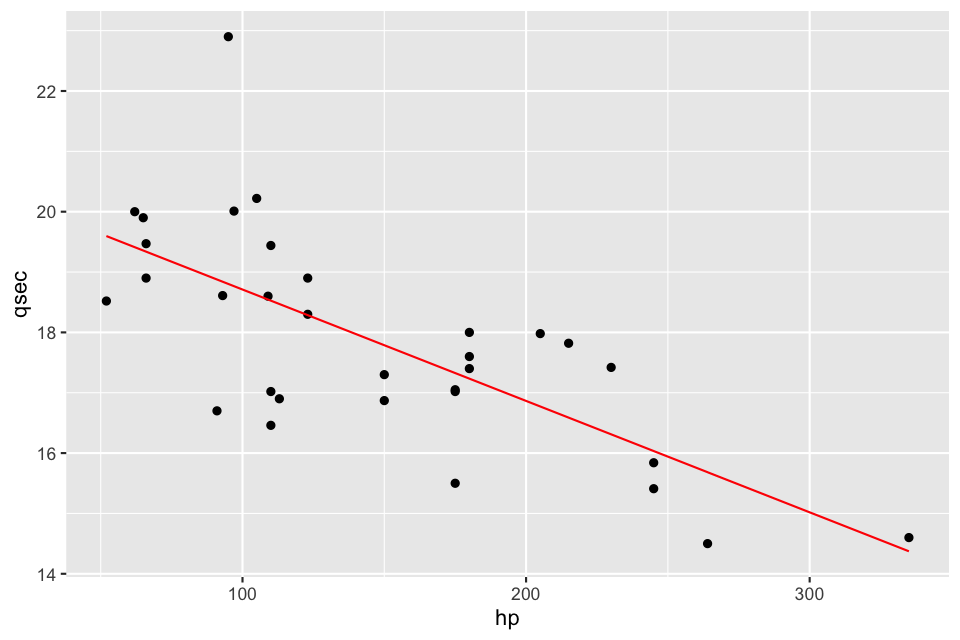
\includegraphics[width=.9\linewidth]{./resources/mtcars_linreg1.png}
\end{center}
\end{org}

Using our visualization in combination with our calculated p-value and r-squared value, we have determined that there is a significant relationship between horsepower and quarter-mile time.

The variability we observed within our horsepower data must come from multiple sources of variance. To accurately predict future horsepower observations, we need to use a more robust model.

\subsection{Multiple Linear Regression}
\label{sec:org7a0c4d4}

Multiple linear regression is a statistical model that extends the scope and flexibility of a simple linear regression model. Instead of using a single independent variable to account for all variability observed in the dependent variable, a multiple linear regression uses multiple independent variables to account for parts of the total variance observed in the dependent variable. For all independent x variables and their m coefficients.

y = m1x1 + m2x2 + ... + mnxn + b

When it comes to multiple linear regression, we'll look at each independent variable to determine if there is a significant relationship with the dependent variable. Once we have evaluated each independent variable, we'll evaluate the r-squared value of the model to determine if the model sufficiently predicts our dependent variable.

\begin{verbatim}
lm(
  qsec ~ mpg + disp + drat + wt + hp,
  data = mtcars
)
\end{verbatim}

\begin{org}


Call:
lm(formula = qsec \textasciitilde{} mpg + disp + drat + wt + hp, data = mtcars)

Coefficients:
(Intercept)          mpg         disp         drat           wt           hp  
  16.541651     0.108579    -0.008076    -0.578953     1.792793    -0.018383
\end{org}

Because multiple linear regression models use multiple variables and dimensions, they are almost impossible to plot and visualize.

We can create a summary.

\begin{verbatim}
summary(
  lm(
    qsec ~ mpg + disp + drat + wt + hp,
    data = mtcars
  )
)
\end{verbatim}

\begin{org}


Call:
lm(formula = qsec \textasciitilde{} mpg + disp + drat + wt + hp, data = mtcars)

Residuals:
    Min      1Q  Median      3Q     Max
-1.6628 -0.6138  0.0706  0.4087  3.3885

Coefficients:
             Estimate Std. Error t value Pr(>|t|)
(Intercept) 16.541651   3.413109   4.847 5.04e-05 \textbf{*}
mpg          0.108579   0.077911   1.394  0.17523
disp        -0.008076   0.004384  -1.842  0.07689 .
drat        -0.578953   0.551771  -1.049  0.30371
wt           1.792793   0.513897   3.489  0.00175 \textbf{*
hp          -0.018383   0.005421  -3.391  0.00223 *}
---
Signif. codes:  0 ‘***’ 0.001 ‘**’ 0.01 ‘*’ 0.05 ‘.’ 0.1 ‘ ’ 1

Residual standard error: 1.053 on 26 degrees of freedom
Multiple R-squared:  0.7085,	Adjusted R-squared:  0.6524
F-statistic: 12.64 on 5 and 26 DF,  p-value: 2.767e-06
\end{org}

The data we want to look for is the one under \textbf{Pr(>|t|)}. Plus the \textbf{p-value} and the \textbf{mutliple R-squared}.

In the summary output, each Pr(>|t|) value represents the probability that each coefficient contributes a random amount of variance to the linear model.

According to our results, vehicle weight and horsepower (as well as intercept) are statistically unlikely to provide random amounts of variance to the linear model. In other words the vehicle weight and horsepower have a significant impact on quarter-mile race time.

When an intercept is statistically significant, it means that the intercept term explains a significant amount of variability in the dependent variable when all independent vairables are equal to zero. Alternatively, it may mean that there are other variables that can help explain the variability of our dependent variable that have not been included in our model.

Despite the number of significant variables, the multiple linear regression model outperformed the simple linear regression.

According to the summary output, the \textbf{r-squared} value has increased from 0.50 in the simple linear regression model to 0.71 in our multiple linear regression model while the \textbf{p-value} remained significant.

As with any data model, it takes practice to learn how to identify variables of interest, select an appropriate model, and refine a model to increase performance.

\section{Category Complexities}
\label{sec:orgd1c5b22}

One common form of categorical data is frequency data, where we record how often something was observed within a single variable. For example, in the mpg dataset, if we were to count up the number of vehicles for each vehicle class, the output would be a form of frequency data.

In data science, we'll often compare frequency data across another dichotomous factor such as gender, A/B groups, member/non-member, and so on. In these cases, we may ask ourselves, ``Is there a difference in frequency between our first and second groups?'' To test this question, we can perform a chi-squared test.

\subsection{Chi-squared test}
\label{sec:org7f25ce7}

The chi-squared test is used to compare the distribution of frequencies across two groups and tests the following hypotheses:

\begin{itemize}
\item H0 : There is no difference in frequency distribution between both groups.
\item Ha : There is a difference in frequency distribution between both groups
\end{itemize}

Before we can perform our chi-squared analysis, we must ensure that our dataset meets the assumptions of the statistical test:

\begin{enumerate}
\item Each subject within a group contributes to only one frequency. In other words, the sum of all frequencies equals the total number of subjects in a dataset.
\item Each unique value has an equal probability of being observed.
\item There is a minimum of five observed instances for every unique value for a 2x2 chi-squared table.
\item For a larger chi-squared table, there is at least one observation for every unique value and at least 80\% of all unique values have five or more observations.
\end{enumerate}

The most straightforward implementation of chisq.test() function is passing the function to a contingency table.

A contingency table is another name for a frequency table produced using R's table() function. R's table() function does all the heavy lifting for us by calculating frequencies across factors.

\begin{verbatim}
table(mpg$class, mpg$year)
\end{verbatim}

\begin{org}
\begin{center}
\begin{tabular}{rr}
1999 & 2008\\
\hline
2 & 3\\
25 & 22\\
20 & 21\\
6 & 5\\
16 & 17\\
19 & 16\\
29 & 33\\
\end{tabular}
\end{center}
\end{org}

Now we use \texttt{chisq.test()}.

\begin{verbatim}
tbl <- table(mpg$class, mpg$year)
chisq.test(tbl)
\end{verbatim}

\begin{org}


Pearson's Chi-squared test

data:  tbl
X-squared = 1.0523, df = 6, p-value = 0.9836

Warning message:
In chisq.test(tbl) : Chi-squared approximation may be incorrect
\end{org}

We were not able to cancel the null hypothesis.

Despite having no quantitative input, the chi-squared test enables data scientists to quantify the distribution of categorical variables.

It's important to keep the number of unique values and groups relatively low. A good rule of thumb is to keep the number of unique values and groups lower than 20, which means the degrees of freedom (df in the output) is less than or equal to 19.

\subsection{AB testing}
\label{sec:org2d5d12d}

To properly evaluate potential product changes, companies can use a technique called A/B testing. A/B testing is a randomized controlled experiment that uses a control (unchanged) and experimental (changed) group to test potential changes using a success metric. A/B testing is used to test whether or not the distribution of the success metric increases in the experiment group instead of the control group; we would not want to make changes to the product that would cause a decrease in the success metric.

First, we must decide what changes will be made to the experimental group. Typically, the number of changes will be very limited to ensure comparisons are equal; however, more substantial changes can also be tested using an A/B framework.

Once a consensus has been made on the changes to be made to the experimental group, a success metric should be determined.

For example, a website might use consumer engagement as a success metric (e.g., number of visitors, clicked links, or time spent on a page).

Once we have decided on our experimental changes and the success metric, we must determine which statistical test is most appropriate.

For our purposes, we can apply the following logic to determine the most appropriate statistical test:

\begin{enumerate}
\item If the success metric is numerical and the sample size is small, a z-score summary statistic can be sufficient to compare the mean and variability of both groups.
\item If the success metric is numerical and the sample size is large, a two-sample t-test should be used to compare the distribution of both groups.
\item If the success metric is categorical, you may use a chi-squared test to compare the distribution of categorical values between both groups.
\end{enumerate}

After determining the testing conditions and statistical test, the next consideration in A/B testing is sample size. It's important to collect a sufficient number of data points for each group to ensure that the A/B test results are meaningful.

Due to its simple design and flexible application, the A/B testing framework is quickly becoming a go-to standard in the data science industry and one of the most highly desired data skills for Fortune 500 companies.

\subsection{Retrospective Analysis}
\label{sec:orgee0cef2}

In data science, researchers use retrospective analysis to analyze and interpret a previously generated dataset where the outcome is already known. Retrospective analyses are helpful because there are no upfront costs to generate data and statistical results can be compared to the known outcomes. Depending on the dataset and input variables, there is a (potentially) limitless number of statistical questions that can be asked from the data:

\begin{enumerate}
\item Are two groups statistically different? Use a t-test with one dichotomous independent variable and one continuous dependent variable.
\item Can one continuous dependent variable be predicted using another independent variable? What about multiple independent variables and one dependent variable? Use regression analysis.
\item Are there multiple categorical variables tightly linked in a dataset? Are the distributions of the different categorical variables equal? We can test with chi-squared.
\end{enumerate}

In contrast, researchers can design their own study to answer their own specific questions. In this case, the data types and size of the dataset will be directly reflective of how complicated their hypotheses are, and what statistical analyses are required to answer the question.

Once we select the variables to collect, we would estimate sample size based on how low of a significance level is necessary and how sensitive the measurements are.

Regardless, if we collect and measure the data ourselves, or if the data has been curated from a previous dataset, statistical tests can help us provide quantitative interpretation to the results.
\end{document}
